% Created by tikzDevice version 0.12.3.1 on 2022-03-16 15:50:08
% !TEX encoding = UTF-8 Unicode
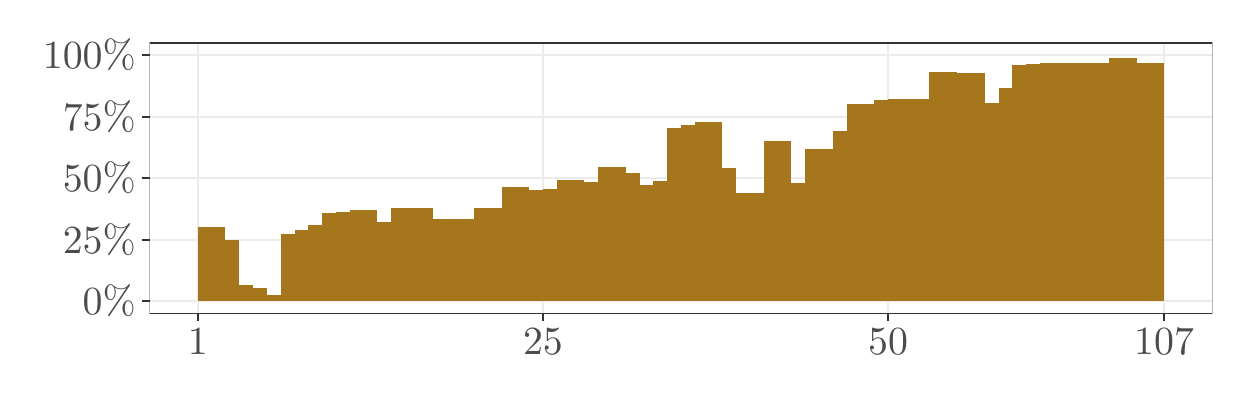
\begin{tikzpicture}[x=1pt,y=1pt]
\definecolor{fillColor}{RGB}{255,255,255}
\path[use as bounding box,fill=fillColor,fill opacity=0.00] (0,0) rectangle (433.62,126.47);
\begin{scope}
\path[clip] (  0.00,  0.00) rectangle (433.62,126.47);
\definecolor{drawColor}{RGB}{255,255,255}
\definecolor{fillColor}{RGB}{255,255,255}

\path[draw=drawColor,line width= 0.6pt,line join=round,line cap=round,fill=fillColor] (  0.00,  0.00) rectangle (433.62,126.47);
\end{scope}
\begin{scope}
\path[clip] ( 44.04, 23.17) rectangle (428.12,120.97);
\definecolor{fillColor}{RGB}{255,255,255}

\path[fill=fillColor] ( 44.04, 23.17) rectangle (428.12,120.97);
\definecolor{drawColor}{gray}{0.92}

\path[draw=drawColor,line width= 0.6pt,line join=round] ( 44.04, 27.61) --
	(428.12, 27.61);

\path[draw=drawColor,line width= 0.6pt,line join=round] ( 44.04, 49.84) --
	(428.12, 49.84);

\path[draw=drawColor,line width= 0.6pt,line join=round] ( 44.04, 72.07) --
	(428.12, 72.07);

\path[draw=drawColor,line width= 0.6pt,line join=round] ( 44.04, 94.30) --
	(428.12, 94.30);

\path[draw=drawColor,line width= 0.6pt,line join=round] ( 44.04,116.53) --
	(428.12,116.53);

\path[draw=drawColor,line width= 0.6pt,line join=round] ( 61.50, 23.17) --
	( 61.50,120.97);

\path[draw=drawColor,line width= 0.6pt,line join=round] (186.20, 23.17) --
	(186.20,120.97);

\path[draw=drawColor,line width= 0.6pt,line join=round] (310.90, 23.17) --
	(310.90,120.97);

\path[draw=drawColor,line width= 0.6pt,line join=round] (410.66, 23.17) --
	(410.66,120.97);
\definecolor{fillColor}{RGB}{166,118,29}

\path[fill=fillColor] ( 61.50, 27.61) rectangle ( 71.48, 54.51);

\path[fill=fillColor] ( 66.49, 27.61) rectangle ( 76.46, 49.92);

\path[fill=fillColor] ( 71.48, 27.61) rectangle ( 81.45, 33.66);

\path[fill=fillColor] ( 76.46, 27.61) rectangle ( 86.44, 32.57);

\path[fill=fillColor] ( 81.45, 27.61) rectangle ( 91.43, 29.93);

\path[fill=fillColor] ( 86.44, 27.61) rectangle ( 96.42, 29.93);

\path[fill=fillColor] ( 91.43, 27.61) rectangle (101.40, 52.09);

\path[fill=fillColor] ( 96.42, 27.61) rectangle (106.39, 53.53);

\path[fill=fillColor] (101.40, 27.61) rectangle (111.38, 55.14);

\path[fill=fillColor] (106.39, 27.61) rectangle (116.37, 59.54);

\path[fill=fillColor] (111.38, 27.61) rectangle (121.36, 59.94);

\path[fill=fillColor] (116.37, 27.61) rectangle (126.34, 60.57);

\path[fill=fillColor] (121.36, 27.61) rectangle (131.33, 56.13);

\path[fill=fillColor] (126.34, 27.61) rectangle (136.32, 55.60);

\path[fill=fillColor] (131.33, 27.61) rectangle (141.31, 61.46);

\path[fill=fillColor] (136.32, 27.61) rectangle (146.30, 61.22);

\path[fill=fillColor] (141.31, 27.61) rectangle (151.28, 57.50);

\path[fill=fillColor] (146.30, 27.61) rectangle (156.27, 56.94);

\path[fill=fillColor] (151.28, 27.61) rectangle (161.26, 57.25);

\path[fill=fillColor] (156.27, 27.61) rectangle (166.25, 57.47);

\path[fill=fillColor] (161.26, 27.61) rectangle (171.24, 61.17);

\path[fill=fillColor] (166.25, 27.61) rectangle (176.22, 48.36);

\path[fill=fillColor] (171.24, 27.61) rectangle (181.21, 68.80);

\path[fill=fillColor] (176.22, 27.61) rectangle (186.20, 51.53);

\path[fill=fillColor] (181.21, 27.61) rectangle (191.19, 67.65);

\path[fill=fillColor] (186.20, 27.61) rectangle (196.18, 68.01);

\path[fill=fillColor] (191.19, 27.61) rectangle (201.16, 71.55);

\path[fill=fillColor] (196.18, 27.61) rectangle (206.15, 70.87);

\path[fill=fillColor] (201.16, 27.61) rectangle (211.14, 69.06);

\path[fill=fillColor] (206.15, 27.61) rectangle (216.13, 76.05);

\path[fill=fillColor] (211.14, 27.61) rectangle (221.12, 74.05);

\path[fill=fillColor] (216.13, 27.61) rectangle (226.10, 65.06);

\path[fill=fillColor] (221.12, 27.61) rectangle (231.09, 69.49);

\path[fill=fillColor] (226.10, 27.61) rectangle (236.08, 71.06);

\path[fill=fillColor] (231.09, 27.61) rectangle (241.07, 90.24);

\path[fill=fillColor] (236.08, 27.61) rectangle (246.06, 91.39);

\path[fill=fillColor] (241.07, 27.61) rectangle (251.05, 92.25);

\path[fill=fillColor] (246.06, 27.61) rectangle (256.03, 75.76);

\path[fill=fillColor] (251.05, 27.61) rectangle (261.02, 66.75);

\path[fill=fillColor] (256.03, 27.61) rectangle (266.01, 66.61);

\path[fill=fillColor] (261.02, 27.61) rectangle (271.00, 66.61);

\path[fill=fillColor] (266.01, 27.61) rectangle (275.99, 85.63);

\path[fill=fillColor] (271.00, 27.61) rectangle (280.97, 69.60);

\path[fill=fillColor] (275.99, 27.61) rectangle (285.96, 70.30);

\path[fill=fillColor] (280.97, 27.61) rectangle (290.95, 82.63);

\path[fill=fillColor] (285.96, 27.61) rectangle (295.94, 71.44);

\path[fill=fillColor] (290.95, 27.61) rectangle (300.93, 89.21);

\path[fill=fillColor] (295.94, 27.61) rectangle (305.91, 98.77);

\path[fill=fillColor] (300.93, 27.61) rectangle (310.90, 90.54);

\path[fill=fillColor] (305.91, 27.61) rectangle (315.89,100.40);

\path[fill=fillColor] (310.90, 27.61) rectangle (320.88,100.54);

\path[fill=fillColor] (315.89, 27.61) rectangle (325.87,100.55);

\path[fill=fillColor] (320.88, 27.61) rectangle (330.85,100.08);

\path[fill=fillColor] (325.87, 27.61) rectangle (335.84,110.48);

\path[fill=fillColor] (330.85, 27.61) rectangle (340.83,110.17);

\path[fill=fillColor] (335.84, 27.61) rectangle (345.82,110.26);

\path[fill=fillColor] (340.83, 27.61) rectangle (350.81, 98.92);

\path[fill=fillColor] (345.82, 27.61) rectangle (355.79, 99.10);

\path[fill=fillColor] (350.81, 27.61) rectangle (360.78,104.85);

\path[fill=fillColor] (355.79, 27.61) rectangle (365.77,112.84);

\path[fill=fillColor] (360.78, 27.61) rectangle (370.76,113.47);

\path[fill=fillColor] (365.77, 27.61) rectangle (375.75,113.77);

\path[fill=fillColor] (370.76, 27.61) rectangle (380.73,113.80);

\path[fill=fillColor] (375.75, 27.61) rectangle (385.72,112.60);

\path[fill=fillColor] (380.73, 27.61) rectangle (390.71,113.82);

\path[fill=fillColor] (385.72, 27.61) rectangle (395.70,109.62);

\path[fill=fillColor] (390.71, 27.61) rectangle (400.69,115.50);

\path[fill=fillColor] (395.70, 27.61) rectangle (405.67,111.98);

\path[fill=fillColor] (400.69, 27.61) rectangle (410.66,113.59);
\definecolor{drawColor}{gray}{0.20}

\path[draw=drawColor,line width= 0.6pt,line join=round,line cap=round] ( 44.04, 23.17) rectangle (428.12,120.97);
\end{scope}
\begin{scope}
\path[clip] (  0.00,  0.00) rectangle (433.62,126.47);
\definecolor{drawColor}{gray}{0.30}

\node[text=drawColor,anchor=base east,inner sep=0pt, outer sep=0pt, scale=  1.44] at ( 39.09, 22.65) {0\%};

\node[text=drawColor,anchor=base east,inner sep=0pt, outer sep=0pt, scale=  1.44] at ( 39.09, 44.88) {25\%};

\node[text=drawColor,anchor=base east,inner sep=0pt, outer sep=0pt, scale=  1.44] at ( 39.09, 67.11) {50\%};

\node[text=drawColor,anchor=base east,inner sep=0pt, outer sep=0pt, scale=  1.44] at ( 39.09, 89.34) {75\%};

\node[text=drawColor,anchor=base east,inner sep=0pt, outer sep=0pt, scale=  1.44] at ( 39.09,111.57) {100\%};
\end{scope}
\begin{scope}
\path[clip] (  0.00,  0.00) rectangle (433.62,126.47);
\definecolor{drawColor}{gray}{0.20}

\path[draw=drawColor,line width= 0.6pt,line join=round] ( 41.29, 27.61) --
	( 44.04, 27.61);

\path[draw=drawColor,line width= 0.6pt,line join=round] ( 41.29, 49.84) --
	( 44.04, 49.84);

\path[draw=drawColor,line width= 0.6pt,line join=round] ( 41.29, 72.07) --
	( 44.04, 72.07);

\path[draw=drawColor,line width= 0.6pt,line join=round] ( 41.29, 94.30) --
	( 44.04, 94.30);

\path[draw=drawColor,line width= 0.6pt,line join=round] ( 41.29,116.53) --
	( 44.04,116.53);
\end{scope}
\begin{scope}
\path[clip] (  0.00,  0.00) rectangle (433.62,126.47);
\definecolor{drawColor}{gray}{0.20}

\path[draw=drawColor,line width= 0.6pt,line join=round] ( 61.50, 20.42) --
	( 61.50, 23.17);

\path[draw=drawColor,line width= 0.6pt,line join=round] (186.20, 20.42) --
	(186.20, 23.17);

\path[draw=drawColor,line width= 0.6pt,line join=round] (310.90, 20.42) --
	(310.90, 23.17);

\path[draw=drawColor,line width= 0.6pt,line join=round] (410.66, 20.42) --
	(410.66, 23.17);
\end{scope}
\begin{scope}
\path[clip] (  0.00,  0.00) rectangle (433.62,126.47);
\definecolor{drawColor}{gray}{0.30}

\node[text=drawColor,anchor=base,inner sep=0pt, outer sep=0pt, scale=  1.44] at ( 61.50,  8.30) {1};

\node[text=drawColor,anchor=base,inner sep=0pt, outer sep=0pt, scale=  1.44] at (186.20,  8.30) {25};

\node[text=drawColor,anchor=base,inner sep=0pt, outer sep=0pt, scale=  1.44] at (310.90,  8.30) {50};

\node[text=drawColor,anchor=base,inner sep=0pt, outer sep=0pt, scale=  1.44] at (410.66,  8.30) {107};
\end{scope}
\end{tikzpicture}
